\documentclass{llncs}
\usepackage[utf8]{inputenc}
\usepackage[spanish]{babel}
\usepackage{amsmath}
\usepackage{graphicx}
\usepackage{booktabs}
\usepackage{float}
\usepackage{placeins}

\renewcommand{\andname}{y}
\renewcommand{\lastandname}{\unskip\ y}

\begin{document}

\title{Cifrado de Im\'agenes Basado en Convoluci\'on en el Dominio de Frecuencia con Derivaci\'on de Clave por Contrase\~na}

\author{M.C. Zuriel L\'opez Sosa \and Dra. B\'arbara Emma S\'anchez Rinza \and
Dr. Carlos Ignacio Robledo S\'anchez}
\institute{Benemerita Universidad Autonoma de Puebla\\
\email{zuriel.lopezs@correo.buap.mx, brinza@fcfm.buap.mx, crobledo@fcfm.buap.mx}}

\maketitle

\begin{abstract}
El cifrado de im\'agenes es fundamental para la comunicaci\'on digital
segura y la protecci\'on de datos visuales. Este trabajo presenta un
m\'etodo de cifrado basado en la Transformada de Fourier (FT), en el cual
tanto la imagen original como una clave, generada criptogr\'aficamente a
partir de una contrase\~na, se transforman al dominio de la frecuencia. La
clave se deriva mediante PBKDF2-HMAC-SHA256 y se expande con SHAKE-256 hasta
el tama\~no exacto de la imagen, eliminando la necesidad de un archivo de
clave externo. El proceso de cifrado aplica la Transformada R\'apida de
Fourier (FFT) a ambas representaciones y las multiplica elemento a elemento;
la imagen cifrada se reconstruye con la Transformada Inversa (IFFT) y se
almacena en un formato PNG de 16 bits por canal con los metadatos de
normalizaci\'on embebidos. Para evaluar la seguridad y efectividad del
m\'etodo se realizaron an\'alisis estad\'isticos (histogramas, entrop\'ia y
PSNR) y pruebas de robustez ante ataques de ruido gaussiano, reescalado y
contrase\~na incorrecta. Los resultados muestran que la imagen cifrada
exhibe alta aleatoriedad y baja correlaci\'on con el original, que el
proceso de descifrado recupera la imagen original de forma exacta
(PSNR infinito) con la contrase\~na correcta, y que el m\'etodo es
sumamente sensible a alteraciones de la clave, del tama\~no de la imagen
cifrada y de la contrase\~na utilizada.

\keywords{Cifrado de imagenes, Transformada de Fourier, seguridad digital,
cifrado en el dominio de frecuencia, derivacion de claves, PBKDF2,
SHAKE-256, analisis criptografico.}
\end{abstract}

\section{Introducci\'on}

En la era digital, la seguridad de la informaci\'on es una prioridad,
especialmente en lo referente a la protecci\'on de im\'agenes, las cuales
suelen contener datos sensibles. Las im\'agenes digitales, por su
naturaleza visual, presentan un reto adicional para los m\'etodos de
cifrado tradicionales centrados en el dominio espacial. Las t\'ecnicas de
cifrado en el dominio de la frecuencia, como las basadas en la Transformada
de Fourier (FT), han ganado atenci\'on por su capacidad de ocultar
eficazmente los patrones de los datos, dificultando el descifrado sin la
clave adecuada \cite{refregier,unnikrishnan}. Entre las alternativas
existentes se encuentran los esquemas de codificaci\'on de fase aleatoria en
el dominio \'optico \cite{javidi} y los esquemas basados en mapas
ca\'oticos \cite{chaos1,chaos2}, que persiguen objetivos similares de
aleatorizaci\'on mediante din\'amicas no lineales en el dominio espacial.

El cifrado de im\'agenes basado en FT, y en particular en la Transformada
R\'apida de Fourier (FFT), ofrece una soluci\'on eficiente al problema de la
protecci\'on de im\'agenes en canales no seguros. Este trabajo presenta un
m\'etodo que transforma tanto la imagen original como una clave al dominio
de la frecuencia y las combina mediante multiplicaci\'on elemento a
elemento. A diferencia de esquemas que requieren distribuir una
imagen-clave junto con los datos cifrados, la clave utilizada aqu\'i se
deriva de una \textbf{contrase\~na} mediante funciones criptogr\'aficas
est\'andar, de manera que \'unicamente se necesitan el archivo cifrado y la
contrase\~na para recuperar la imagen original, en l\'inea con las nociones
formales de seguridad criptogr\'afica que exigen que un atacante sin la
clave correcta no pueda distinguir la salida del cifrado de ruido aleatorio
\cite{bellare}.

El objetivo de este art\'iculo es presentar y evaluar dicho m\'etodo,
examinando su efectividad y seguridad. La evaluaci\'on de desempe\~no se
realiza mediante pruebas estad\'isticas (comparaci\'on de histogramas,
entrop\'ia y PSNR) y pruebas de robustez ante posibles ataques.

La estructura de este art\'iculo es la siguiente: la Secci\'on 2 describe el
algoritmo propuesto, detallando el proceso de cifrado y descifrado. La
Secci\'on 3 presenta las pruebas realizadas y el an\'alisis de resultados.
Finalmente, la Secci\'on 4 concluye con una discusi\'on de los hallazgos.

\section{Metodolog\'ia}

El algoritmo se basa en la \textbf{propiedad de convoluci\'on de la
Transformada de Fourier}, que establece que la transformada de Fourier de
la convoluci\'on de dos funciones es igual al producto de sus respectivas
transformadas:
\[
\mathcal{F}(f * g) = \mathcal{F}(f) \cdot \mathcal{F}(g)
\]
Aislando el t\'ermino de convoluci\'on y aplicando la Transformada Inversa
de Fourier ($\mathcal{F}^{-1}$) en ambos lados se obtiene:
\[
f * g = \mathcal{F}^{-1}\left(\mathcal{F}(f) \cdot \mathcal{F}(g)\right)
\]
Esto implica que la convoluci\'on en el dominio espacial puede calcularse
indirectamente mediante multiplicaci\'on en el dominio de la frecuencia,
seguida de la Transformada Inversa. En la pr\'actica, ambas transformadas se
calculan mediante el algoritmo de la Transformada R\'apida de Fourier (FFT)
\cite{cooley}, que reduce la complejidad del c\'alculo de $O(N^2)$ a
$O(N\log N)$.

A lo largo de este art\'iculo, $f$ denota la \textbf{imagen original} a
cifrar y $g$ denota la \textbf{imagen-clave}. El cifrado se define como la
convoluci\'on $f * g$: dicha convoluci\'on, calculada en el dominio de la
frecuencia como se describi\'o arriba, \textbf{es} la imagen cifrada. Para
recuperar la imagen original basta despejar $f$ de la propiedad de
convoluci\'on, dividiendo en el dominio de la frecuencia por
$\mathcal{F}(g)$ en lugar de multiplicar:
\[
f = \mathcal{F}^{-1}\left(\frac{\mathcal{F}(f * g)}{\mathcal{F}(g)}\right)
\]
Esta es precisamente la relaci\'on que instancian, respectivamente, el
proceso de cifrado (Secci\'on~2.2) y el de descifrado (Secci\'on~2.3):
el primero produce $f*g$ a partir de $f$ y $g$; el segundo recupera $f$ a
partir de $f*g$ y $g$. Dado que las im\'agenes utilizadas son RGB, todas
las operaciones se realizan de forma independiente en cada uno de los tres
canales de color (Rojo, Verde y Azul), es decir, $f$, $g$ y $f*g$ se tratan
canal por canal.

\subsection{Derivaci\'on de la clave $g$ a partir de una contrase\~na}

En lugar de requerir que $g$ provenga de una imagen-clave externa, $g$ se
genera criptogr\'aficamente a partir de una contrase\~na. Este dise\~no
sigue el principio de Kerckhoffs \cite{kerckhoffs}, seg\'un el cual la
seguridad de un sistema criptogr\'afico debe residir \'unicamente en el
secreto de la clave (aqu\'i, la contrase\~na) y no en el secreto del
algoritmo ni en la posesi\'on de un archivo adicional. La derivaci\'on
sigue el mismo principio que emplean los cifradores de flujo modernos y las
funciones de derivaci\'on de claves basadas en contrase\~nas
\cite{nist800132,scrypt}: derivar una clave corta y expandirla en un flujo
pseudoaleatorio del tama\~no necesario.

\begin{enumerate}
  \item Se genera un \emph{salt} aleatorio de 16 bytes en el momento del
    cifrado.
  \item La contrase\~na y el \emph{salt} se procesan con
    \textbf{PBKDF2-HMAC-SHA256} \cite{pbkdf2} usando 310{,}000 iteraciones,
    obteniendo 32 bytes derivados.
  \item Esos 32 bytes se expanden con \textbf{SHAKE-256} (funci\'on de
    salida extensible de la familia SHA-3 \cite{sha3}) hasta obtener
    exactamente $\text{alto}\times\text{ancho}\times 3$ bytes: esos bytes
    constituyen $g$, generada exactamente a las dimensiones de $f$, sin
    necesidad de redimensionamiento.
\end{enumerate}

\subsection{Proceso de cifrado: obtenci\'on de $f*g$}

\begin{enumerate}
  \item \textbf{Entradas}: la imagen original $f$ a cifrar y una
    contrase\~na.
  \item \textbf{Derivaci\'on de la clave}: se obtiene $g$ como se describi\'o
    en la secci\'on anterior.
  \item \textbf{Transformada de Fourier}: se aplica la FFT a cada canal de
    $f$ y de $g$, obteniendo $\mathcal{F}(f)$ y $\mathcal{F}(g)$.
  \item \textbf{Multiplicaci\'on elemento a elemento}: se calcula
    $\mathcal{F}(f)\cdot\mathcal{F}(g)$.
  \item \textbf{Transformada Inversa de Fourier}: se aplica la IFFT al
    resultado anterior, obteniendo $f*g$ en el dominio espacial.
  \item \textbf{Normalizaci\'on y almacenamiento}: se aplica normalizaci\'on
    Min-Max por canal a $f*g$ para llevar sus valores a un rango de 16 bits
    ($[0,65535]$), ya que el resultado de la convoluci\'on tiene un rango
    de valores mucho mayor que el de una imagen convencional. El m\'inimo y
    m\'aximo usados, junto con el \emph{salt} y el n\'umero de iteraciones,
    se embeben como metadatos dentro del propio archivo PNG cifrado (en un
    \emph{chunk} \texttt{tEXt} en formato JSON), de manera que el archivo
    resultante --- que contiene $f*g$ cuantizada a 16 bits --- es
    autocontenido. Este archivo es la \textbf{imagen cifrada}.
\end{enumerate}

\subsection{Proceso de descifrado: recuperaci\'on de $f$ a partir de $f*g$}

\begin{enumerate}
  \item \textbf{Entradas}: la imagen cifrada (que contiene $f*g$
    cuantizada a 16 bits) y la contrase\~na.
  \item \textbf{Lectura de metadatos}: se extraen del propio archivo el
    \emph{salt}, el n\'umero de iteraciones y los rangos min/max de cada
    canal.
  \item \textbf{Re-derivaci\'on de la clave}: se repite el proceso de la
    Secci\'on~2.1 con el mismo \emph{salt}, regenerando $g$ de forma
    id\'entica a la usada en el cifrado.
  \item \textbf{Inversi\'on de la normalizaci\'on}: se convierten los
    valores de 16 bits de vuelta a la escala real de $f*g$, usando los
    rangos almacenados.
  \item \textbf{Transformada de Fourier}: se aplica la FFT a $f*g$ (ya
    desnormalizada) y a $g$, obteniendo $\mathcal{F}(f*g)$ y
    $\mathcal{F}(g)$.
  \item \textbf{Divisi\'on elemento a elemento}: se recupera $f$ dividiendo
    ambas representaciones en el dominio de la frecuencia:
    \[
    f \approx \mathcal{F}^{-1}\left(\frac{\mathcal{F}(f * g)}{\mathcal{F}(g) + \epsilon}\right)
    \]
    con $\epsilon = 1\times10^{-10}$ para evitar divisiones por cero. El
    resultado de esta operaci\'on es la \textbf{imagen descifrada}.
  \item \textbf{Redondeo y recorte}: el resultado se redondea y recorta al
    rango v\'alido $[0,255]$ para obtener la imagen final en 8 bits.
\end{enumerate}

El formato de almacenamiento resultante corresponde a una imagen de 16
bits por canal, capaz de representar el rango completo de valores
requerido por la normalizaci\'on descrita.

\section{An\'alisis y Evaluaci\'on de Desempe\~no}

Esta secci\'on presenta el an\'alisis y la evaluaci\'on de desempe\~no del
m\'etodo propuesto. La evaluaci\'on se realiz\'o sobre una fotograf\'ia de
prueba de $3024\times4032$ p\'ixeles, y consiste en tres etapas: inspecci\'on
visual, an\'alisis estad\'istico y pruebas de robustez ante ataques.

\subsection{Inspecci\'on visual}

\begin{figure}[htbp]
  \centering
  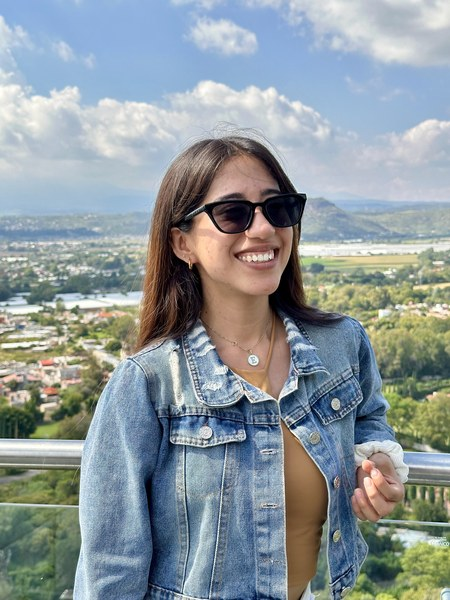
\includegraphics[width=0.3\textwidth]{eval_original.jpg}
  \hfill
  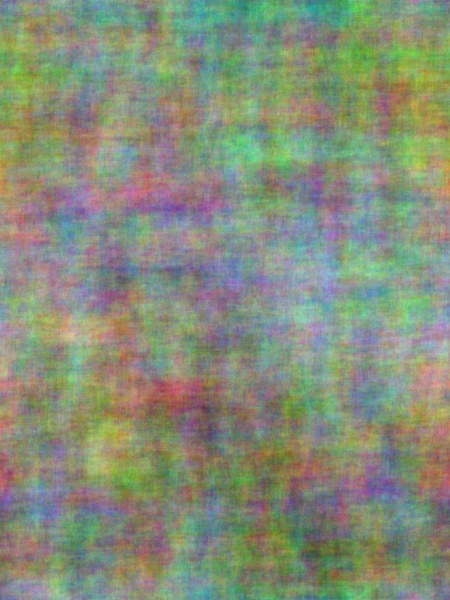
\includegraphics[width=0.3\textwidth]{eval_encrypted.jpg}
  \hfill
  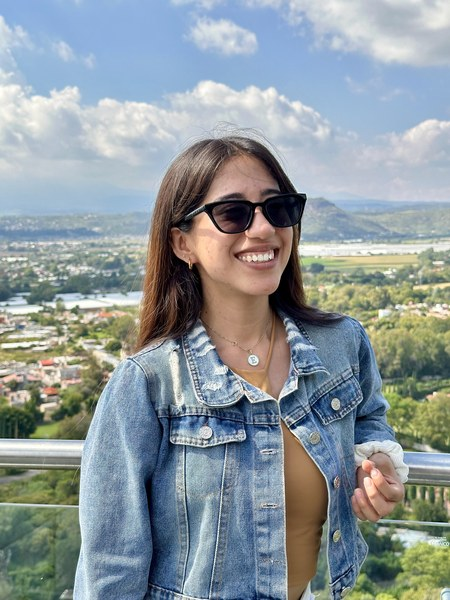
\includegraphics[width=0.3\textwidth]{eval_correct.jpg}
  \caption{De izquierda a derecha: imagen original $f$, imagen cifrada
  $f*g$ (vista previa de 8 bits de los datos reales de 16 bits) e imagen
  descifrada (recuperaci\'on de $f$) tras el descifrado con la
  contrase\~na correcta.}
\end{figure}
\FloatBarrier

La imagen cifrada $f*g$ no muestra ning\'un rasgo reconocible del contenido
de $f$, mientras que la imagen descifrada es, como se cuantifica en la
Secci\'on~3.3, id\'entica a $f$.

\subsection{An\'alisis estad\'istico}

\subsubsection{An\'alisis de histogramas.}
Los histogramas de intensidad son una herramienta est\'andar para analizar
la distribuci\'on de valores de p\'ixel de una imagen \cite{gonzalez}. Se
calcularon los histogramas de $f$ y de $f*g$ para cada canal de color
(Fig.~2). El histograma de la imagen original
presenta picos pronunciados asociados a regiones de color uniforme (cielo,
piel, ropa). El histograma de la imagen cifrada, en cambio, adopta una
forma unimodal suave de tipo gaussiano, consistente con el teorema del
l\'imite central aplicado a la convoluci\'on de dos se\~nales
estad\'isticamente independientes: la estructura de picos del original
desaparece por completo, lo cual indica que el proceso de cifrado oculta
eficazmente la distribuci\'on de intensidades original.

\begin{figure}[htbp]
  \centering
  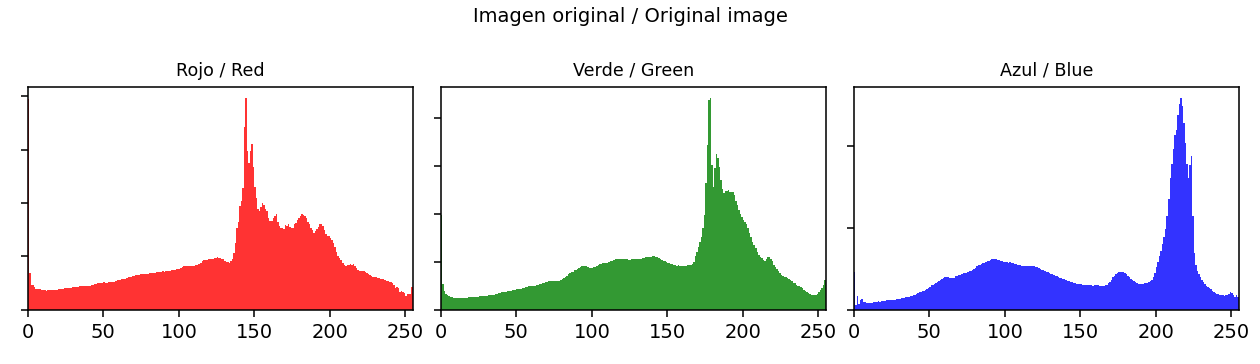
\includegraphics[width=0.9\textwidth]{hist_original.png}\\[4pt]
  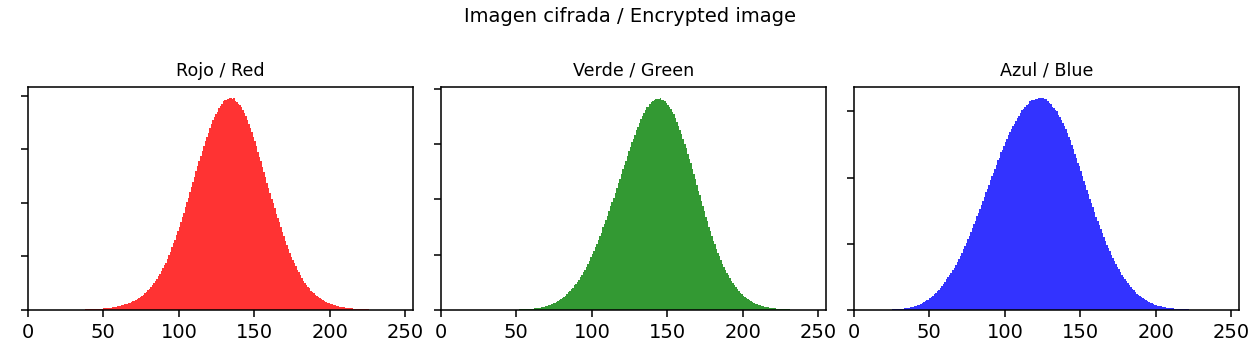
\includegraphics[width=0.9\textwidth]{hist_encrypted.png}
  \caption{Histogramas por canal (R, G, B) de la imagen original (arriba) y
  de la imagen cifrada (abajo).}
\end{figure}
\FloatBarrier

\subsubsection{An\'alisis de entrop\'ia.}
La entrop\'ia de Shannon \cite{shannon} promedio (sobre los tres canales)
de $f$ es de $7.6512$, mientras que la de $f*g$ es de $6.7715$. Esta ligera disminuci\'on, tambi\'en observada en otros esquemas
de cifrado basados en FT, se explica porque la normalizaci\'on Min-Max
concentra los valores en una campana en lugar de saturar uniformemente los
256 niveles posibles; no obstante, la entrop\'ia se mantiene alta, lo que
confirma que el cifrado produce una imagen con alta aleatoriedad aparente.

\subsubsection{Evaluaci\'on de PSNR.}
Se calcul\'o la relaci\'on se\~nal-a-ruido de pico (PSNR) \cite{psnr} entre
$f$ y la imagen recuperada al descifrar $f*g$ con la contrase\~na correcta. El
resultado obtenido fue:
\[
\text{MSE} = 0.0 \qquad \text{PSNR} = \infty
\]
Es decir, la imagen recuperada es \textbf{id\'entica bit a bit} a la
original. Esto confirma que, al usar 16 bits por canal con los rangos de
normalizaci\'on almacenados como metadatos exactos, el proceso de cifrado y
descifrado no introduce ninguna p\'erdida de informaci\'on.

\subsection{Robustez ante ataques}

Adem\'as de las pruebas de histograma, entrop\'ia y PSNR, la literatura de
cifrado de im\'agenes eval\'ua frecuentemente la sensibilidad al p\'ixel
mediante pruebas de aleatoriedad como NPCR y UACI \cite{npcr}. En este
trabajo se opt\'o por evaluar directamente la robustez del esquema frente a
tres ataques concretos: ruido gaussiano, reescalado y contrase\~na
incorrecta.

\subsubsection{Ataque de ruido gaussiano.}
Se agreg\'o ruido gaussiano directamente a $f*g$ (los datos cifrados de 16
bits),
con tres niveles de desviaci\'on est\'andar ($\sigma$) expresados como
fracci\'on del rango de 16 bits ($0.05\%$, $0.25\%$ y $0.5\%$, equivalentes
a $\sigma \approx 32.8$, $163.8$ y $327.7$ en unidades de 16 bits). Los
resultados se muestran en la Fig.~3 y la Tabla~1.

\begin{figure}[htbp]
  \centering
  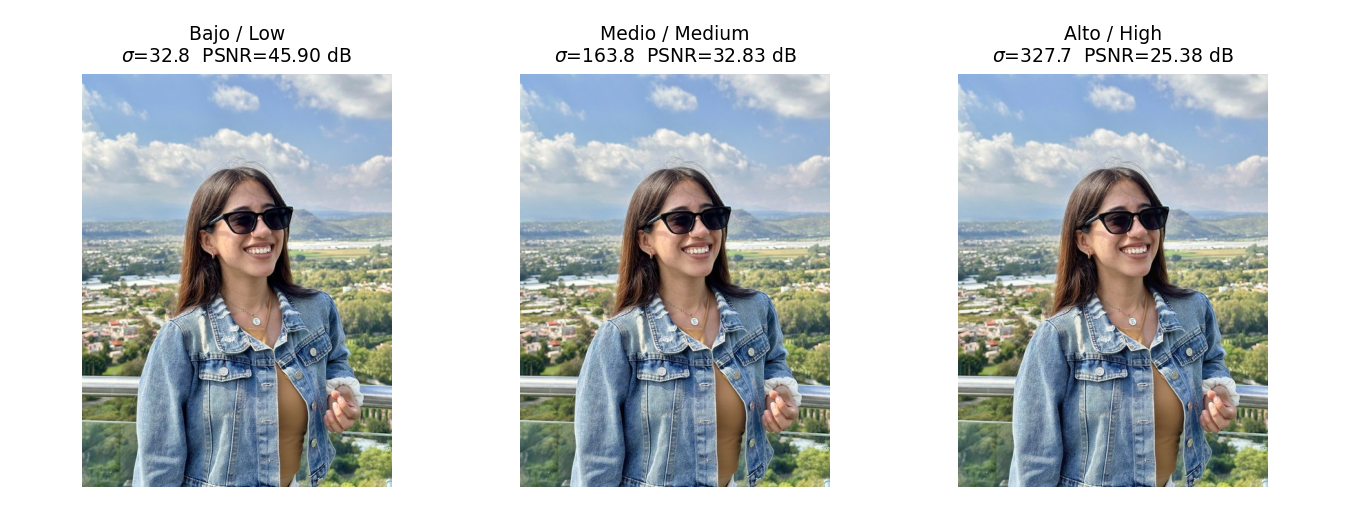
\includegraphics[width=\textwidth]{grid_noise.png}
  \caption{Imagen descifrada tras agregar ruido gaussiano de nivel bajo,
  medio y alto al archivo cifrado, con su PSNR correspondiente.}
\end{figure}
\FloatBarrier

\begin{table}[htbp]
  \centering
  \caption{PSNR de la imagen descifrada tras el ataque de ruido gaussiano.}
  \begin{tabular}{@{}lccc@{}}
    \toprule
    \textbf{Nivel} & \textbf{$\sigma$ (16 bits)} & \textbf{MSE} & \textbf{PSNR (dB)} \\
    \midrule
    Bajo   & 32.8  & 1.67   & 45.90 \\
    Medio  & 163.8 & 33.92  & 32.83 \\
    Alto   & 327.7 & 188.43 & 25.38 \\
    \bottomrule
  \end{tabular}
\end{table}
\FloatBarrier

Como es de esperarse, a mayor nivel de ruido el PSNR disminuye. Sin
embargo, incluso en el nivel m\'as alto probado la imagen recuperada sigue
siendo claramente reconocible (Fig.~3), lo que indica que el m\'etodo
tolera razonablemente perturbaciones peque\~nas del archivo cifrado sin
perder la utilidad de la imagen recuperada.

\subsubsection{Ataque de reescalado.}
Se evalu\'o el efecto de aplicar interpolaci\'on bilineal para modificar la
escala de $f*g$ (de 16 bits) antes de descifrar (regenerando $g$ al nuevo
tama\~no en cada caso, ya que $g$ se deriva determin\'isticamente a partir
de la contrase\~na y las dimensiones de la imagen).

\emph{Reducci\'on de escala.} Se redujo $f*g$ al 1\%, 5\% y
10\% de su tama\~no original. En los tres casos, el descifrado
result\'o en una imagen \textbf{completamente saturada} (todos los p\'ixeles
en blanco, valor 255; Fig.~4). Esto se explica porque el t\'ermino de
frecuencia cero (la componente de continua) de los datos cifrados
conserva una magnitud asociada al tama\~no original de la imagen, mientras
que la clave se regenera a una escala mucho menor; el desajuste entre
ambas magnitudes provoca que el resultado de la divisi\'on en frecuencia
se desborde y sature al recortarse al rango $[0,255]$.

\begin{figure}[htbp]
  \centering
  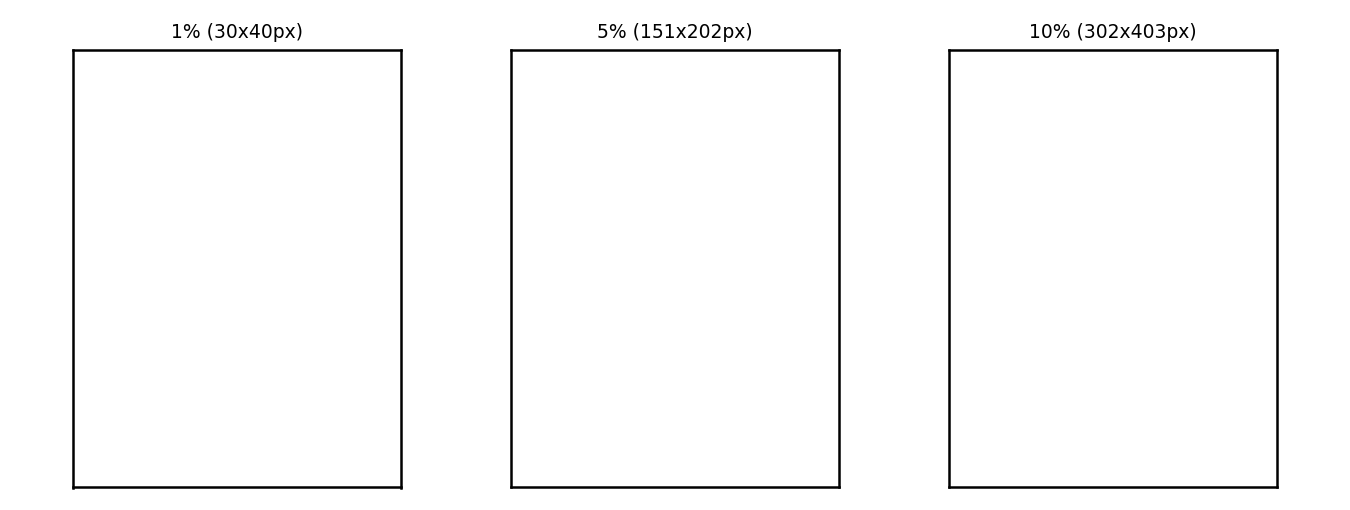
\includegraphics[width=\textwidth]{grid_downscale.png}
  \caption{Resultado del descifrado tras reducir la imagen cifrada al 1\%,
  5\% y 10\% de su tama\~no original: saturaci\'on total (blanco) en los
  tres casos.}
\end{figure}
\FloatBarrier

\emph{Aumento de escala.} Se aument\'o la imagen cifrada en 1\%, 5\% y 10\%.
En los tres casos el resultado fue ruido de color completamente
irreconocible (Fig.~5), sin ning\'un rasgo del contenido original. La
interpolaci\'on introduce artefactos que alteran la representaci\'on en el
dominio de la frecuencia, impidiendo el descifrado correcto.

\begin{figure}[htbp]
  \centering
  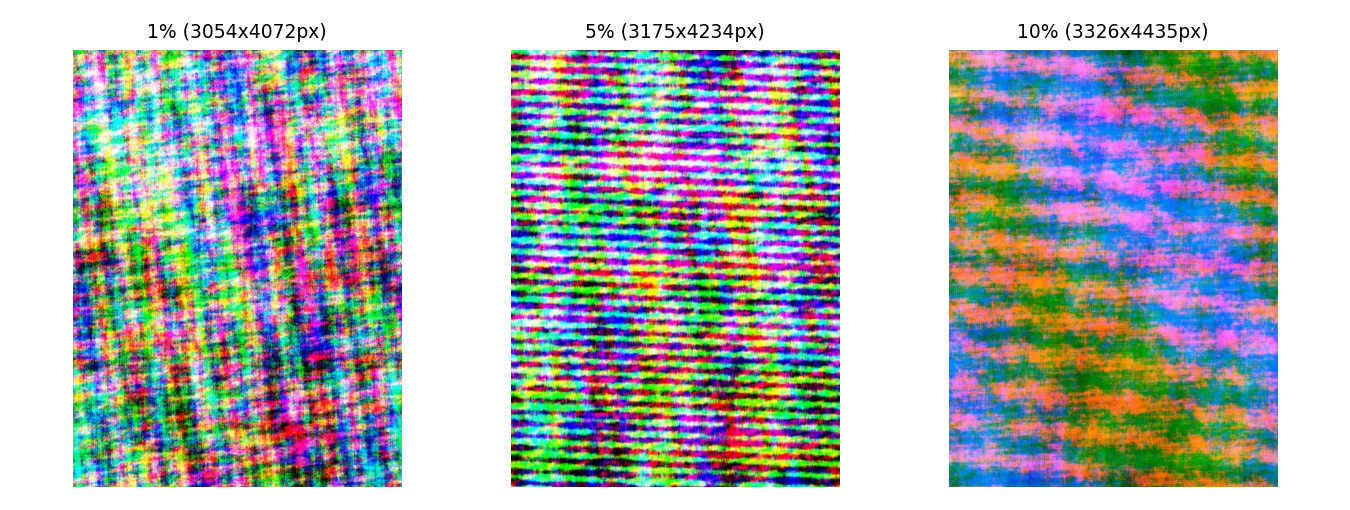
\includegraphics[width=\textwidth]{grid_upscale.png}
  \caption{Resultado del descifrado tras aumentar la imagen cifrada en 1\%,
  5\% y 10\%: ruido irreconocible en los tres casos.}
\end{figure}
\FloatBarrier

En ambos casos (reducci\'on y aumento de escala), el m\'etodo demuestra ser
altamente sensible a cualquier alteraci\'on geom\'etrica del archivo
cifrado, una propiedad deseable para detectar manipulaciones no
autorizadas.

\subsubsection{Descifrado con contrase\~na incorrecta.}
Se intent\'o descifrar la imagen usando una contrase\~na distinta a la
utilizada en el cifrado. El resultado, mostrado en la Fig.~6, es ruido de
color completamente irreconocible:
\[
\text{MSE} = 13727.85 \qquad \text{PSNR} = 6.75~\text{dB}
\]

\begin{figure}[htbp]
  \centering
  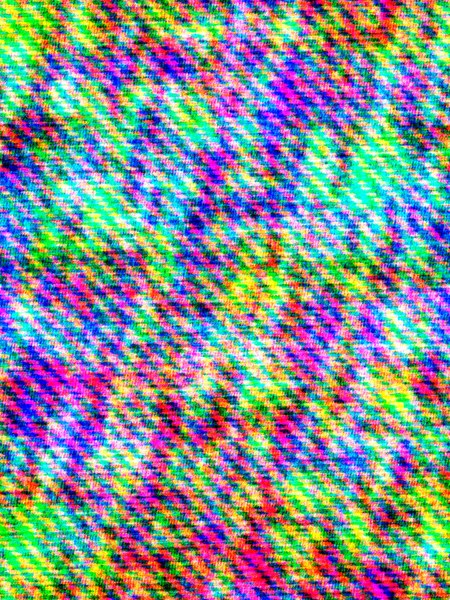
\includegraphics[width=0.32\textwidth]{eval_wrong_password.jpg}
  \caption{Resultado de intentar descifrar la imagen con una contrase\~na
  incorrecta.}
\end{figure}
\FloatBarrier

Este resultado confirma que el esquema depende de forma cr\'itica de la
contrase\~na exacta: incluso una contrase\~na distinta produce una
reconstrucci\'on totalmente inutilizable, reforzando la seguridad del
m\'etodo.

\section{Conclusiones}

El an\'alisis demuestra que el m\'etodo de cifrado basado en convoluci\'on
en el dominio de frecuencia, con clave derivada de una contrase\~na,
transforma eficazmente el contenido de una imagen en una representaci\'on
de apariencia aleatoria, dif\'icil de distinguir visual y
estad\'isticamente del ruido. Las evaluaciones estad\'isticas confirman una
alta entrop\'ia y una p\'erdida total de la estructura de histograma
original en la imagen cifrada, mientras que el descifrado con la
contrase\~na correcta recupera la imagen original de forma \textbf{exacta}
(PSNR infinito), a diferencia de esquemas equivalentes basados en
normalizaci\'on de 8 bits, que introducen p\'erdida irreversible de
informaci\'on.

Las pruebas de robustez muestran que el m\'etodo tolera niveles moderados de
ruido gaussiano manteniendo una imagen recuperada reconocible, pero es
extremadamente sensible a transformaciones geom\'etricas (reescalado) y a
cualquier desviaci\'on en la contrase\~na utilizada, ambas propiedades
deseables para detectar manipulaciones no autorizadas del archivo cifrado.
En conjunto, el esquema ofrece un nivel de seguridad s\'olido, eliminando
adem\'as la necesidad de distribuir un archivo de clave externo, lo cual lo
hace pr\'actico para transmisi\'on segura de im\'agenes.

\begin{thebibliography}{16}
\bibitem{refregier} Refregier, P., Javidi, B.: Optical image encryption
  based on input plane and Fourier plane random encoding. Optics Letters
  20(7), 767--769 (1995).
\bibitem{unnikrishnan} Unnikrishnan, G., Joseph, J., Singh, K.: Optical
  encryption system that uses phase conjugation in a photorefractive
  crystal. Applied Optics 37(35), 8181--8186 (1998).
\bibitem{javidi} Javidi, B., Zhang, G., Li, J.: Experimental demonstration of
  the random phase encoding technique for image encryption and security
  verification. Optical Engineering 35(9), 2506--2512 (1996).
\bibitem{chaos1} Chen, G., Mao, Y., Chui, C.K.: A symmetric image encryption
  scheme based on 3D chaotic cat maps. Chaos, Solitons \& Fractals 21(3),
  749--761 (2004).
\bibitem{chaos2} Zhou, Y., Bao, L., Chen, C.L.P.: A new 1D chaotic system for
  image encryption. Signal Processing 97, 172--182 (2014).
\bibitem{cooley} Cooley, J.W., Tukey, J.W.: An algorithm for the machine
  calculation of complex Fourier series. Mathematics of Computation 19(90),
  297--301 (1965).
\bibitem{kerckhoffs} Kerckhoffs, A.: La cryptographie militaire. Journal des
  sciences militaires 9, 5--38 (1883).
\bibitem{pbkdf2} Moriarty, K., Kaliski, B., Rusch, A.: PKCS \#5: Password-Based
  Cryptography Specification, Version 2.1. RFC 8018 (2017).
\bibitem{nist800132} Turan, M.S., Barker, E., Burr, W., Chen, L.:
  Recommendation for Password-Based Key Derivation, Part 1: Storage
  Applications. NIST Special Publication 800-132 (2010).
\bibitem{scrypt} Percival, C.: Stronger key derivation via sequential
  memory-hard functions. In: BSDCan 2009 (2009).
\bibitem{sha3} National Institute of Standards and Technology: SHA-3 Standard:
  Permutation-Based Hash and Extendable-Output Functions. FIPS PUB 202 (2015).
\bibitem{shannon} Shannon, C.E.: A mathematical theory of communication. The
  Bell System Technical Journal 27(3), 379--423 (1948).
\bibitem{gonzalez} Gonzalez, R.C., Woods, R.E.: Digital Image Processing,
  4th ed. Pearson (2018).
\bibitem{psnr} Hore, A., Ziou, D.: Image quality metrics: PSNR vs. SSIM. In:
  20th International Conference on Pattern Recognition (ICPR), pp.
  2366--2369 (2010).
\bibitem{npcr} Wu, Y., Noonan, J.P., Agaian, S.: NPCR and UACI randomness
  tests for image encryption. Cyber Journals: Journal of Selected Areas in
  Telecommunications, 31--38 (2011).
\bibitem{bellare} Bellare, M., Desai, A., Pointcheval, D., Rogaway, P.:
  Relations among notions of security for public-key encryption schemes. In:
  CRYPTO 1998, LNCS 1462, pp. 26--45 (1998).
\end{thebibliography}

\end{document}
